\chapter{Android Application}
\section {Overview}
The application was designed to allow the users to interact with the blockchain. The Application UI was made similar to modern social networks, displaying the nearby events as a scrollable home feed \hyperref[fig:appscreens]{Figure 4.1} shows the different screens design of the Android app.  Authentication is required for the user to login to the blockchain network and to use the app. Once the user login
\ \\
 \begin{figure}[H]
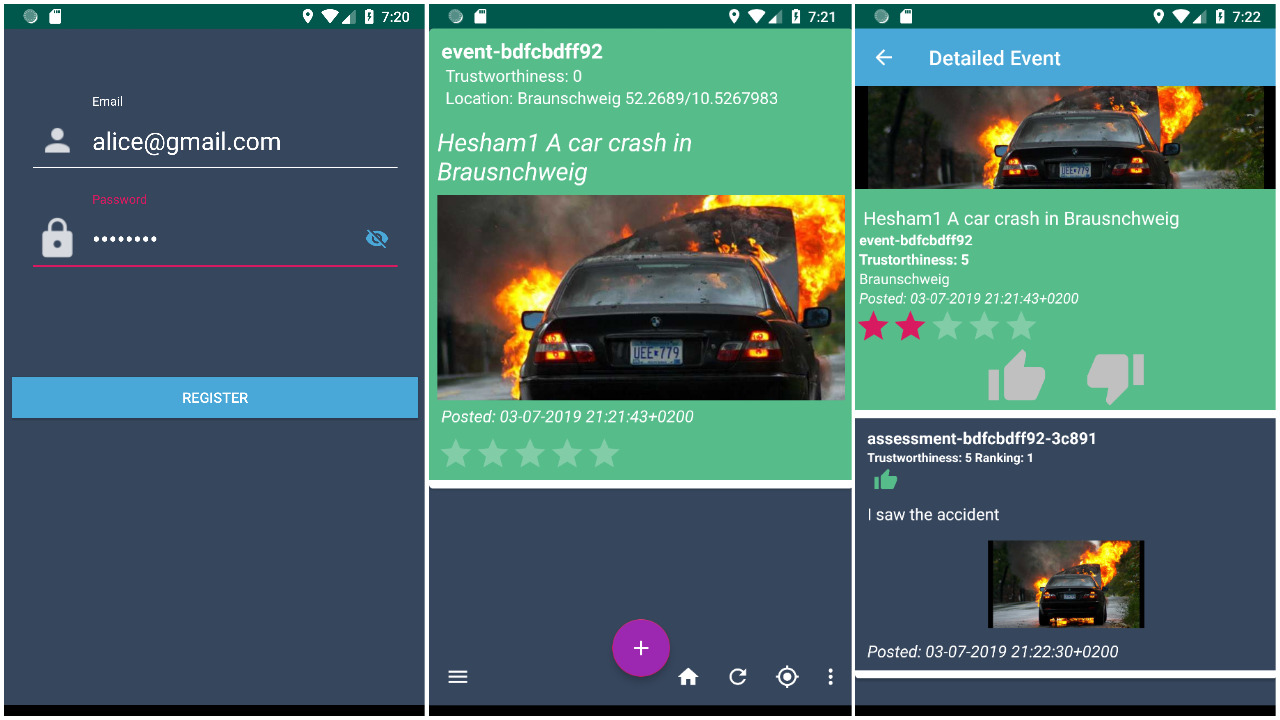
\includegraphics[width=15cm,height=10cm]{images/appscreens.jpg}
\caption{App Screens represent the application design}
\label{fig:appscreens}
\end{figure}
 
\section{The Main Classes} 

In this section, we describe the main classes we used in the application. Every class provided a different functionality.
\subsection{Mainactivity}
MainActiivty is the main activity launched when the application started. it checks if the user logged-in then it will direct the user to registration and login activity. 
Once the user login the email address will be stored in the shared-preference in order to keep the user login. The location access permission will be checked as it's one of the essential parts to fetch the location of the users. A warning message will be displayed to the user if the location access wasn't guaranteed. As long as the location is guaranteed. An enrollment request will be sent using the user's email address as discussed in the enrollment procedures 3.6 and storing the JWT for making blockchain requests. 
Finally, the application will use the JWT and the user's location to query the ledger and fetch all the nearby events and displaying them one by one chronologically in the news feed. 
Displaying the feed is nontrivial we used RecyclerView.An adapter is an android class used to represent the data dynamically in a separate view. in another word every time we query the ledger the user get a JSON response of all event list. those events will be displayed individually every one in a separate view. 
we create a simple view holder for every event object and we instantiate an object of this view holder and bind the event data to it.    
The Same methdology used to displaying the assessments list.
\hyperref[fig:mainactivityflow]{Figure 4.2} Describes the flow of the Mainactivity. 
 \begin{figure}[H]
\center
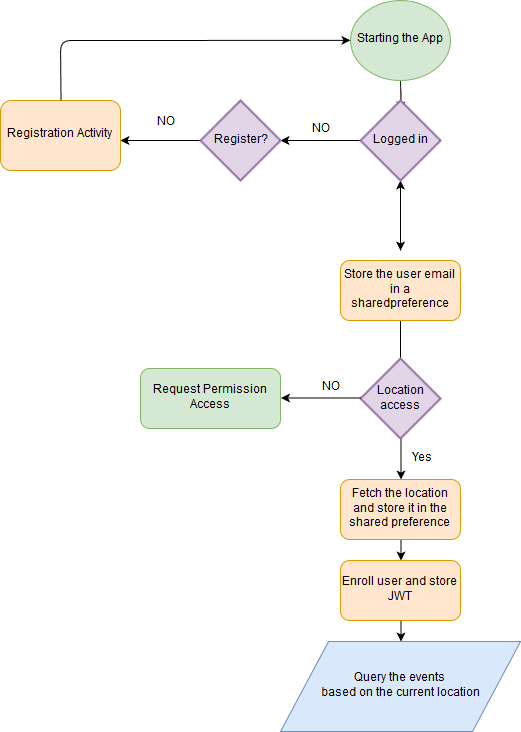
\includegraphics[width=10cm,height=11cm]{images/mainactivityflow.png}
\caption{Mainactivity Flowchart}
\label{fig:mainactivityflow}
\end{figure}

\subsection{AddEvent}
AddEvent is the activity that runs when the user wanted to add an event it will prompt the user to upload a photo and an event description. the activity will check the storage's permission access, and if it's guaranteed it will allow the user to select an image from the gallery, then the image will be captured as a bitmap and converted into string .this string will be hashed and stored on the server. so the picture will be stored with its hash and only the hash will be stored on the blockchain. Storing the hash instead of the entire media file will be more efficient as the file will be replicated many times on the peers. thus storing the hash only will save a lot of disk space.    
\hyperref[fig:mainactivityflow]{Figure 4.3} Describes the flow of AddingEvent Activity. 
 \begin{figure}[H]
\center
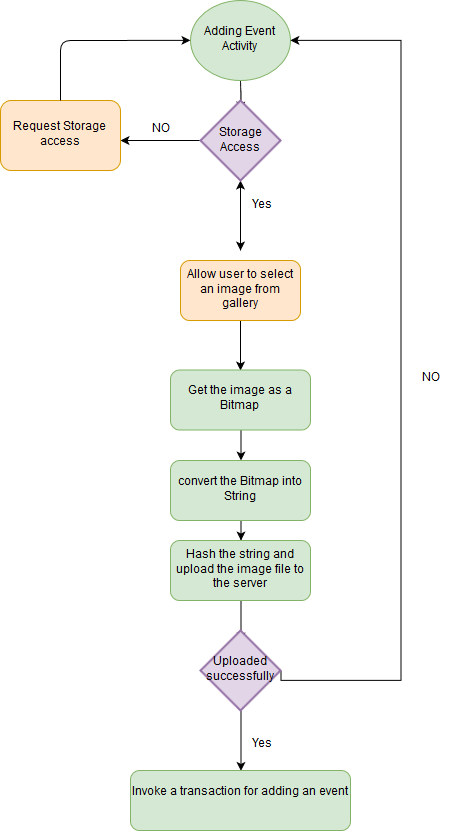
\includegraphics[width=10cm,height=13cm]{images/addingeventflowchart.png}
\caption{Addevent Flowchart}
\label{fig:addingeventflowchart}
\end{figure}

\subsection{Voting}
When the user selects on a specific event a new activity created displaying more details about the events and allow the user to judge or assesses the events by upvoting or downvoting and attaching a description or a media file. Assessing events will credit or discredit the event and directly reflects the users' reputation. 

\subsection{The Hashing Method}
For a more efficient way of storing data on the blockchain, only the media file is hashed and only the hash of it will be stored on CDN like S3 we store the data on a simple Xampp server for development purpose. the media file will be easily fetched and displayed. 
\textbf{PBKDF2} Algorithm is implemented. this hash function is slow enough to impede attacks, but still fast enough to not cause a noticeable delay for the user. A simple implemenetation of the hashing algorithm in listing 4.1.

 \begin{lstlisting}[caption={PBKDF2 Simple Implementation},captionpos=b]
import javax.crypto.SecretKeyFactory;
import javax.crypto.spec.PBEKeySpec;
import java.math.BigInteger;

public class Hashing {

    private static final int ITERATIONS = 1000;
    private static final int KEY_LENGTH = 192; // bits
    public static final String SALT = "Random Salt" ;

    public static String hashPassword(String password, String salt){
        char[] passwordChars = password.toCharArray();
        byte[] saltBytes = salt.getBytes();

        PBEKeySpec spec = new PBEKeySpec(
                passwordChars,
                saltBytes,
                ITERATIONS,
                KEY_LENGTH
        );
        SecretKeyFactory key = null;
        try {
            key = SecretKeyFactory.getInstance("PBKDF2WithHmacSHA1");
        } catch (NoSuchAlgorithmException e) {
            e.printStackTrace();
        }
        byte[] hashedPassword = new byte[0];
        try {
            hashedPassword = key.generateSecret(spec).getEncoded();
        } catch (InvalidKeySpecException e) {
            e.printStackTrace();
        }
        return String.format("%x", new BigInteger(hashedPassword));
    }

}
\end{lstlisting}
\cleardoublepage

\subsection{Login and Register}
In order to allow the users to log in and register, we implemented two separate activities. the user will input an email and password we are validating the user input. and an error will be displayed if the email address is not valid or empty or in use by another user. 
If the data was valid we submit a request over the network and store it to the relational database. The email will be stored in a plain text, however, the password will be stored hashed. 
Similarly, the login activity once the user inputs his email and password it will be checked against the database if the credentials were correct the access is granted to the user and the email will be saved to keep the user logged in.


\subsection{Ranking and Trustworithness} 

One of the main features we introduced is ranking the events and calculating users' reputation.
The user's reputation will depend on the user's interaction on the platform. how frequent he participated, how many good reviews he received. 
Every user starts with 0 reputation score. Adding an event will increase his score by +1. 
The algorithm considers the users rank and location trustworthiness or how close is the user from the event.
As shown in the figure  
Assume a user with score 510 and was about 10 m from an event he is going to assess. first, we convert the score into stars as the user's reputation score is 510 then the stars function will return function. second, we calculate how far is the use and return a value from 1(almost in the event he is assessing ) to .1(so far away from the event) in this case the closeness function will emit 1 so the final score the user is 25. This score will increase/decrease the event, which this user assesses depending on the vote type if it's up/down vote this will credit or discredit the event. 
In summary, What easily influences the user’s reputation is getting good/bad reviews from the highly ranked users. 
\hyperref[fig:mainactivityflow]{Figure 4.4} Describes the ranking algorithm. 
 \begin{figure}[H]
\center
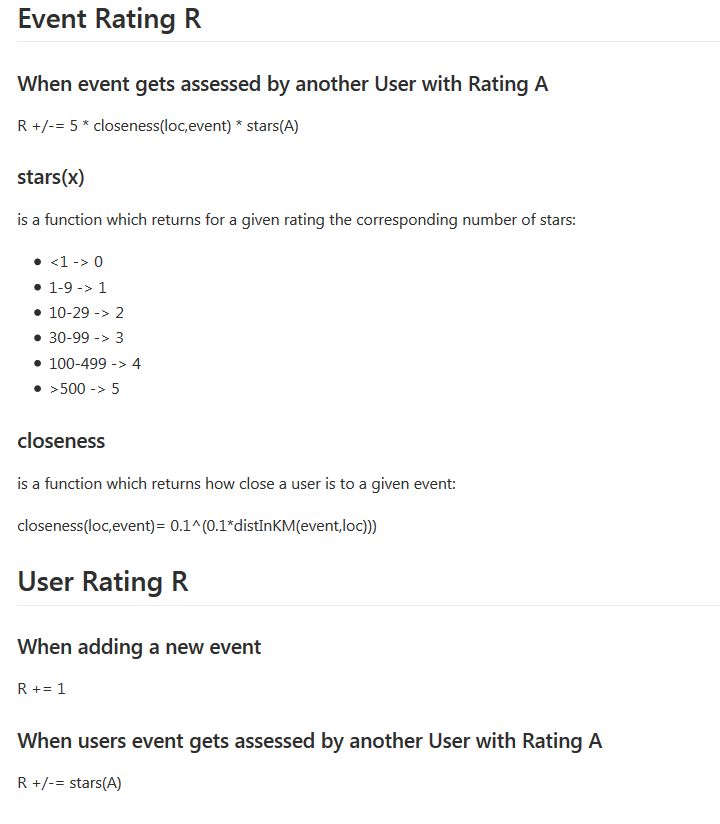
\includegraphics[width=12cm,height=10cm]{images/ranking.png}
\caption{The Ranking Algorithm}
\label{fig:ranking}
\end{figure}
 
 






 



 
  